\documentclass[11pt,a4paper]{article}
\usepackage[a4paper, margin=1.3in]{geometry}
\usepackage{mathtools}
\usepackage{fancyhdr}
\usepackage{mathrsfs}

\newcommand{\sheetNr}{9}

\pagestyle{fancy}
\fancyhf{}
\lhead{AI Planning}
\rhead{Exercise Sheet \sheetNr}
\lfoot{Axel Perschmann, Tarek Saier, \today}
\rfoot{Page \thepage\ of \pageref{lastpage}}
\renewcommand{\headrulewidth}{0.3pt}
\renewcommand{\footrulewidth}{0.3pt}
\setlength\parindent{0pt}
\newcommand{\h}[0]{\text{--}}

\begin{document}
\begin{center}
\Huge{\textbf{AI Planning}}\\
\LARGE{\textbf{Exercise Sheet \sheetNr}}
\end{center}
\vspace{2cm}
\begin{tabular}{ll}
Date: & \today\\
Students: & Axel Perschmann, Tarek Saier
\end{tabular}

\section*{Exercise 9.1}
\textbf{(a)} Compatibility graph:\\
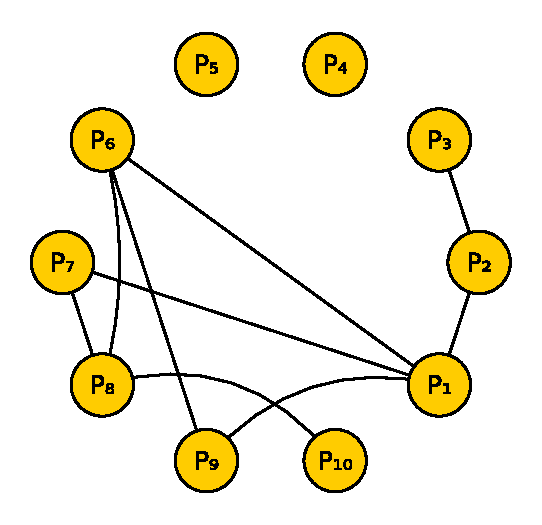
\includegraphics[scale=0.7]{compgraph}\\
Maximal cliques: $\{P_1,P_2\}$, $\{P_1,P_6,P_9\}$, $\{P_1,P_7\}$, $\{P_2,P_3\}$, $\{P_4\}$, $\{P_5\}$, $\{P_6,P_8\}$, $\{P_7,P_8\}$, $\{P_8,P_{10}\}$.\\
\\
\textbf{(b)}\\
\\
\textbf{(c)}\\

\label{lastpage}
\end{document}
